
% 
% Annual Cognitive Science Conference
% Sample LaTeX Paper -- Proceedings Format
% 

% Original : Ashwin Ram (ashwin@cc.gatech.edu)       04/01/1994
% Modified : Johanna Moore (jmoore@cs.pitt.edu)      03/17/1995
% Modified : David Noelle (noelle@ucsd.edu)          03/15/1996
% Modified : Pat Langley (langley@cs.stanford.edu)   01/26/1997
% Latex2e corrections by Ramin Charles Nakisa        01/28/1997 
% Modified : Tina Eliassi-Rad (eliassi@cs.wisc.edu)  01/31/1998
% Modified : Trisha Yannuzzi (trisha@ircs.upenn.edu) 12/28/1999 (in process)
% Modified : Mary Ellen Foster (M.E.Foster@ed.ac.uk) 12/11/2000
% Modified : Ken Forbus                              01/23/2004
% Modified : Eli M. Silk (esilk@pitt.edu)            05/24/2005
% Modified : Niels Taatgen (taatgen@cmu.edu)         10/24/2006
% Modified : David Noelle (dnoelle@ucmerced.edu)     11/19/2014

%% Change ''letterpaper'' in the following line to ''a4paper'' if you must.

\documentclass[10pt,letterpaper]{article}

\usepackage{cogsci}
\usepackage{pslatex}
\usepackage{apacite}
\usepackage{amsmath,amssymb}
\usepackage{graphicx}
\usepackage{color}
\usepackage{url}
\usepackage{todonotes}
\usepackage{mathtools}
\usepackage{stmaryrd}
\usepackage{booktabs}
\usepackage{array}
\graphicspath{{./figures/}}

%\newcommand{\url}[1]{$#1$}

\definecolor{Red}{RGB}{255,0,0}
\newcommand{\red}[1]{\textcolor{Red}{#1}}
\definecolor{Green}{RGB}{10,200,100}
\newcommand{\ndg}[1]{\textcolor{Green}{[ndg: #1]}}


 \newcommand{\denote}[1]{\mbox{ $[\![ #1 ]\!]$}}


\newcommand{\subsubsubsection}[1]{{\em #1}}
\newcommand{\eref}[1]{(\ref{#1})}
\newcommand{\tableref}[1]{Table \ref{#1}}
\newcommand{\figref}[1]{Fig.~\ref{#1}}
\newcommand{\appref}[1]{Appendix \ref{#1}}
\newcommand{\sectionref}[1]{Section \ref{#1}}

\title{Learning to communicate about abstractions}
 
\author{{\large \bf Robert X.D. Hawkins \textsuperscript{1}, Michael Franke\textsuperscript{2}, Kenny Smith\textsuperscript{3}, Noah D.~Goodman\textsuperscript{1}} \\
   \textsuperscript{1}Department of Psychology, Stanford University (\{rxdh,ngoodman\}@stanford.edu) \\
  \textsuperscript{2}Department of Linguistics, University of T\"ubingen (mchfranke@gmail.com)\\
  \textsuperscript{3}Centre for Language Evolution, University of Edinburgh (Kenny.Smith@ed.ac.uk)}

\begin{document}

\maketitle


\begin{abstract}
\todo[inline]{TODO: finish abstract} A remarkable feature of our language is the existence of abstract feature of natural languages is What shapes the ? In addition to several qualitative measures of differences in the lexical conventions that emerge, we introduce a model-based approach to infer participants' developing lexica throughout the game. 
\end{abstract}

\section{Introduction}
%% Set up problem
Natural languages provide speakers with remarkable flexibility in the labels they may use to refer to things \cite{Brown58_HowShallAThingBeCalled,Cruse77_PragmaticsLexicalSpecificity}. In addition to the combinatorial explosion of modifiers afforded by compositionality \cite{Partee95_LexicalSemanticsCompositionality}, we have a number of overlapping and nested terms in our lexicon. \emph{Fido}, \emph{Dalmatian}, \emph{dog}, and \emph{animal} can all reasonably be used to talk about the same entity at different levels of abstraction. How these overlapping meanings are learned, and why speakers choose different levels of specificity in different contexts, is increasingly well-understood \cite<e.g.>{XuTenenbaum07_WordLearningBayesian,GrafEtAl16_BasicLevel} but there remains a more fundamental question about the structure of our lexicon: how do abstractions become lexicalized in the first place? %And why do we have words for some abstractions but not for others?

%% Overview of big-picture optimal expressivity theory suggesting an answer
One functional answer is suggested by recent computational approaches to language evolution, which have argued that the lexical conventions of languages balance simplicity, or learnability, with the communicative needs of their users. This optimal expressivity hypothesis accounts well for the lexical distributions found in natural languages across semantic domains like color words and kinship categories \cite{RegierKempKay15_WordMeaningsEfficientCommunication}, as well as the compositional systems that emerge under iterated learning with communication in the lab \cite{WintersKirbySmith14_LanguagesAdapt, KirbyTamarizCornishSmith15_CompressionCommunication}. A key prediction is that the lexicon of a group should be sensitive to the pragmatic demands of their environment. For example, languages in warm regions ought to be more likely to collapse the distinction between ice and snow into a single word, and this prediction is borne out in the data \cite{RegierCarstensenKemp16_WordsForSnow}. 

%% Hypothesis & limitations of past studies
Following this logic, we expect that abstractions are more likely to be lexicalized when making distinctions is less useful. There are several limitations to the current evidence for this hypothesis. First, the most comprehensive evidence is observational, aggregated at the level of overall language statistics as opposed to directly manipulating the contextual conditions of individual language users. 
Second, previous experimental studies have largely focused on the end results, illuminating \emph{why} different systems form under different contexts, as opposed to the process of \emph{how} these optimal systems are arrived at dynamically by interacting, learning agents.

%% Make the case for zooming into dyadic convention formation
While globally shared conventions of a language are shaped over the multi-generational timescales of cultural evolution, contextual pressures operate on the shorter timescales of dyadic interaction. In a matter of minutes, communication partners coordinate on efficient but informative local conventions, or conceptual pacts, for the task at hand \cite{ClarkWilkesGibbs86_ReferringCollaborative, BrennanClark96_ConceptualPactsConversation,HawkinsFrankGoodman17_ConventionFormation}. To understand how \emph{languages} are globally shaped by communicative constraints, it may therefore be valuable to understand the local conventions rapidly formed by adaptive cognitive agents over the course of extended interaction.

Here, we developed an experimental paradigm to examine the causal factors driving the emergence of lexical conventions in real-time interaction. Pairs of participants played a repeated reference game in which they interactively developed an artificial language from scratch \cite<e.g.>{GalantucciGarrod11_ExperimentalSemiotics}. We fixed a set of stimuli in a conceptual hierarchy and manipulated contextual pressure across pairs. In addition to finding positive evidence for the optimal expressivity hypothesis, we conducted a Bayesian Data Analysis of a rational communication model to infer the underlying lexica participants were using throughout the game. This analysis suggests learning mechanisms by which pragmatic agents make different inferences about the lexicon in different contexts, and therefore get away with extending terms more broadly when the context allows.  % rational communication model allowing us to analyze not just what system they converged on but how it got there. % present a learning mechanism at the level of individual agents 
%Here, we show how the statistics of the communicative environment shape which levels of abstraction are lexicalized by interacting agents. 


% Repeated reference games 
%In this paper, however, we show that just as communicative pressures for informativity can lead to the lexicalization of specific names when fine distinctions must be drawn, conceptual abstractions become lexicalized precisely when meaning is under-constrained by context. If there are multiple rabbits around, the travelers may need a specific conventionalized term for each; otherwise, they can achieve the same communicative success with fewer words by learning generalizations. When the pragmatics of the context allow for ambiguity in the intended level of reference, adaptive speakers can get away with extending the term more broadly. 


%% Example that sets up our specific hypothesis?

%Suppose, mixing thought experiments from \citeA{Wittgenstein09_PhilosophicalInvestigations} and \citeA{Quine13_WordAndObject}, that two travelers meet in a forest, with no language in common. One is cooking dinner, and the other agrees to help in exchange for food and shelter. What kind of micro-language do they coordinate on to solve this joint task, and how is it shaped by context? 
%To test intuitions about how pragmatics and context might affect the communication system they develop, we consider two cases. If there are multiple rabbits around, the travelers may need a specific conventionalized term for each; otherwise, they can achieve the same communicative success with fewer words by learning generalizations. 
			
\section{Methods}

\begin{figure*}[t]
\begin{center}
{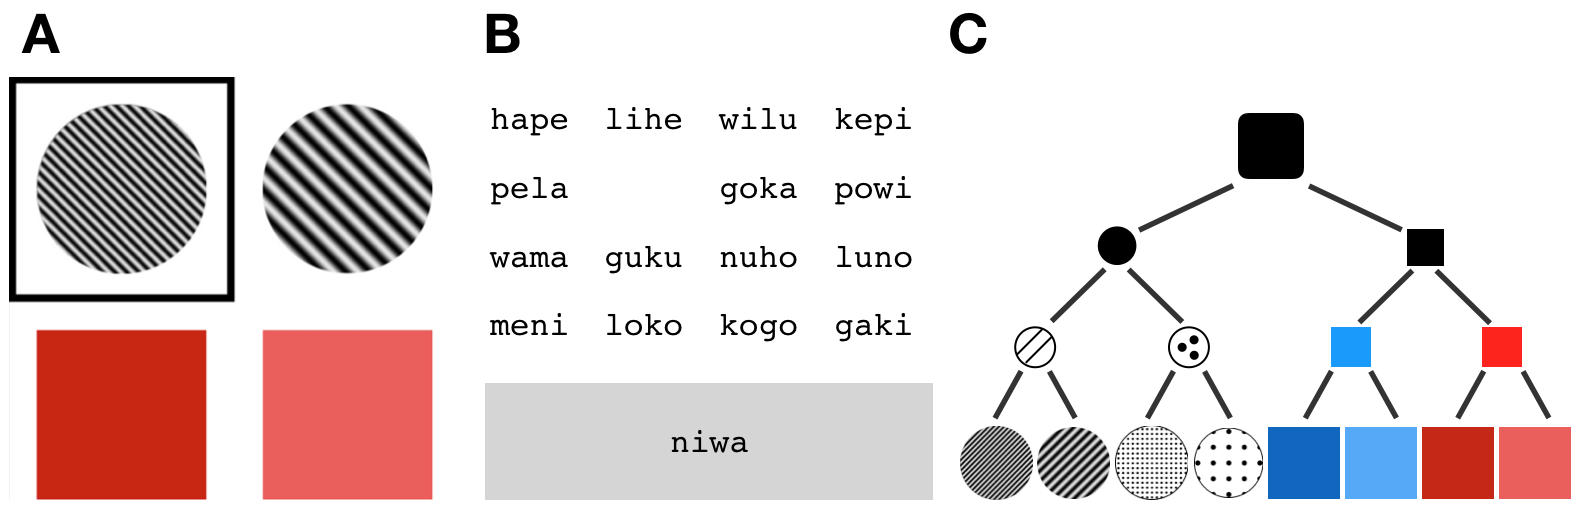
\includegraphics[scale=.65]{fig.png}}
{\caption{{(A) Example array of elements the matcher must choose from. The target is highlighted for the speaker with a black square. In this \emph{subordinate-required} trial there is a distractor at the same intermediate level (striped circle) as the target, so using any abstract label would be insufficient. (B) Drag-and-drop chat box interface. (C) Hierarchical organization of stimuli, with shape at the top-level and color/texture at intermediate levels.  \label{exp}}}}
\end{center}
\end{figure*}

\subsection{Methods}
\subsubsection{Participants}

We recruited 278 participants from Amazon Mechanical Turk to play an interactive, multi-player game using the framework described in \citeA{Hawkins15_RealTimeWebExperiments}. Pairs were randomly assigned to one of three different conditions, yielding between $n=36$ and $n=53$ dyads per condition, after excluding participants who disconnected before completion.

\subsubsection{Stimuli}
The objects that served as referents were designed to cluster in a fixed three-level hierarchy with shape at the top-most level, and color/texture at the intermediate levels (see Fig. 1C). Each communicative context contained four objects. Distractors could differ from the target at various level of the hierarchy, creating different types of contexts defined by the finest distinction that had to be drawn. We focus on two: \emph{subordinate-neighbor} trials, where the closest distractor belongs to the same subordinate category (e.g. a lighter shade of blue square; see Fig. 1A), and \emph{intermediate-neighbor} trials, where the closest distractor belongs to the same intermediate category (e.g. red square instead of blue square). Fixed arrays of 16 utterances were randomly generated in each game by stringing together consonant-vowel pairs into pronounceable 2-syllable words.

\subsubsection{Procedure}
Participants were paired over the web and placed in a shared environment containing an array of four objects (Fig. 1A) and a `chatbox' to send messages from a randomly generated vocabulary (Fig. 1B). On each of 96 trials, one player -- the `speaker' -- was privately shown a highlighted target object and allowed to send a single word to communicate the identity of this object to their partner, who subsequently made a selection from the array. Players swapped roles each round and were rewarded with bonus payment when the listener successfully chose the intended object.

Critically, we manipulated the statistics of the context in a between-subjects design to test the effect of communicative relevance on lexicalization. In the \emph{pure subordinate} condition, all trials had a subordinate-neighbor context; in the \emph{pure intermediate} condition, all trials had a intermediate-neighbor context; in the \emph{mixed} condition, these two contexts were equally likely, thus providing some diversity in the relevant distinctions that must be drawn. Sequences of trials were constructed by randomly shuffling targets and trial types within blocks and ensuring no target appeared more than once in a row.

In addition to behavioral responses collected over the course of the game, we designed a post-test to explicitly probe players' final lexica. For each word, we asked players to select all objects that word can refer to, and for each object, we asked players to select all words that can refer to it. These measures allow us to distinguish between subordinate terms that apply to only one element and abstract terms that apply to all elements belonging to an intermediate level of the hierarchy: striped circles, for example.

\subsection{Behavioral Results}

\subsubsection{People successfully learn to communicate}

Although participants began with no common basis for label meanings, most pairs were nonetheless able to coordinate on a successful communication system over repeated interaction (see Fig. \ref{fig:accuracy}). 
Accuracy improves significantly over the course of the experiment in all conditions ($b = 0.04, p < 0.001$). 
Accuracy also differs significantly \emph{across} conditions: participants in the \emph{pure intermediate} condition performed better throughout the game than participants in the other two conditions who were required to make finer distinctions [stat]. 
Looking more closely at games in the \emph{mixed} condition, we also found that performance on intermediate trials improved \emph{before} subordinate trials %\todo[inline]{Include this plot?} 
Finally, the reaction time taken by the speaker to choose an utterance also decreases significantly over the course of the game, indicating that the lexical mappings may be  [stat]. \todo[inline]{Refine how to say this\dots}

Still, the accuracy distribution was multi-modal: a subpopulation of 29 games (4 from the intermediate condition, 10 from the mixed condition, and 15 from the subordinate condition) still showed relatively poor  performance (i.e. below 75\%) in the fourth quarter. For the subsequent analyses, we exclude these games to ensure we are examining successful lexica.

\subsubsection{Context affects lexicon size}

We predicted that in contexts where speakers were not often required to draw fine distinctions at low levels of the conceptual hierarchy they would develop abstractions applying to everything below a particular node. One coarse consequence of this effect is on lexicon size: we found that participants in the pure intermediate condition reported meanings for significantly fewer words in the post-test ($m = 6.5$) than participants in the mixed and pure subordinate conditions ($b = 2.8, t = 5.0, p <0.001$ and $b = 3.2, t = 4.8, p < 0.001$, respectively). 

\subsubsection{Context affects lexicon content}

\todo[inline]{Omnibus histogram (0,1,2,3,4) collapsing across pairs}
\todo[inline]{Diversity of strategies across pairs}
\todo[inline]{Don't exclude 0}

If participants in the intermediate-only condition can get away with fewer words in their lexicon, what are the meanings of the words they do have? We counted the numbers of specific or holistic terms (e.g. words that refer to only one object) and abstract terms (e.g. words that refer to multiple objects) in the post-test. We found that the likelihood of lexicalizing abstractions differed systematically across conditions (see Fig. \ref{fig:lexiconContent}). Participants in the pure subordinate condition reported lexica containing only specific terms, while participants in the pure intermediate condition reported significantly more abstract terms ($m = 2.5$ \textbf{stat}). The mixed condition lay in between, indicating graded pressure to develop specific terms at the cost of abstract terms. 

These data also reveal an interesting asymmetry in lexicon content across conditions: while abstractions are entirely absent from the pure subordinate condition, specific terms often coexist with abstract terms in the other conditions. In the pure intermediate condition, for instance, participants could in principle perform optimally with only four abstract terms and no subordinate terms. While this was the modal system that emerged (reported in the post-test by nearly 1/3 of participants), abstract terms often coexisted with specific terms. Indeed, the average entropy of the distribution of abstract vs. specific terms within each participant's lexicon was highest in the pure intermediate condition ($m = 0.20$ \textbf{stat}). 

\begin{figure}[t]
\begin{center}
{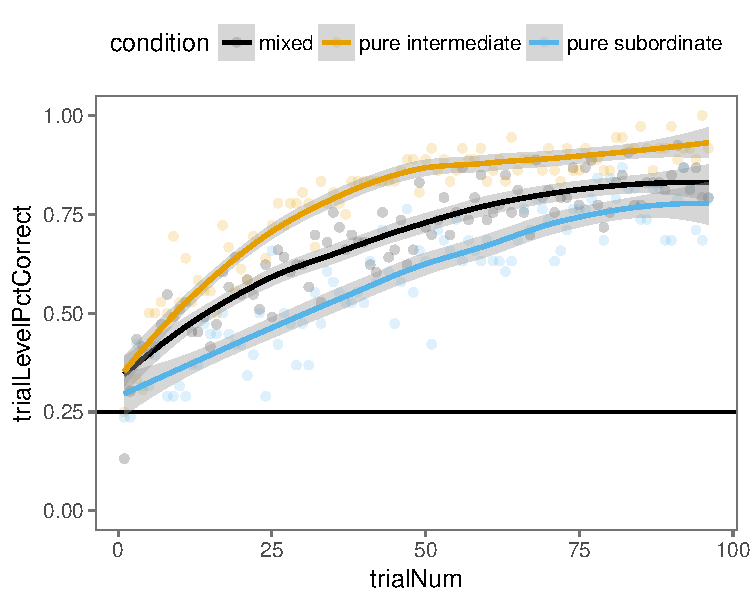
\includegraphics[scale=0.6]{accuracyByCondition.pdf}}
%{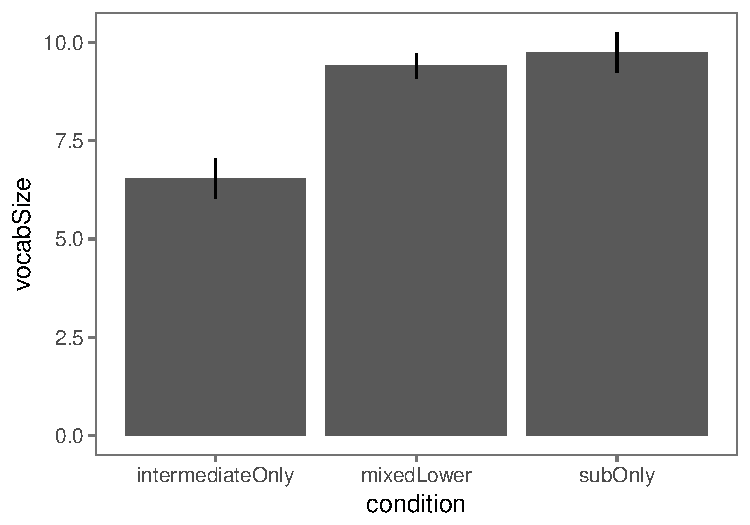
\includegraphics[scale=.64]{lexiconSize.pdf}}
{\caption{{\footnotesize \todo[inline]{TODO: Fix font size, y label; bootstrap error bars instead of SE; 'quartile'}   \label{fig:accuracy}}}}
\end{center}
\end{figure}

\begin{figure}[t]
\begin{center}
{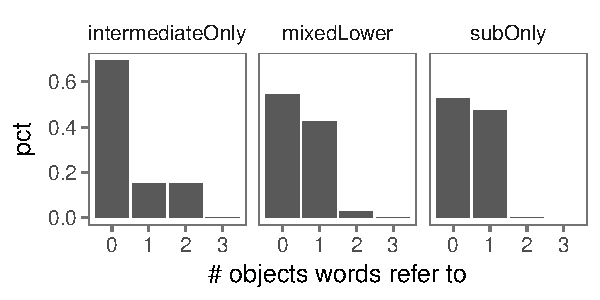
\includegraphics[scale=.64]{lexiconContent.pdf}}
%{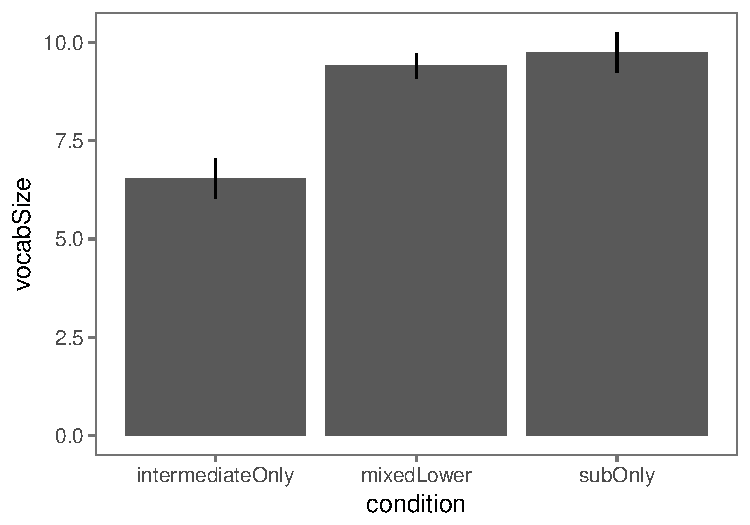
\includegraphics[scale=.64]{lexiconSize.pdf}}
{\caption{{\footnotesize \todo[inline]{TODO: Fix conditions; labels; bootstrap}  \label{fig:lexiconContent}}}}
\end{center}
\end{figure}
\section{Model-based Analysis}

Our post-test provides some insight into the end-result of lexicalization under different communicative contexts, but understanding the \emph{dynamics} of lexicalization requires finer-grained analysis of behavioral trajectories. How do lexica shift and develop over the course of interaction? A recent cognitive model of convention formation has explained the rapid coordination on efficient but informative lexical terms as a process of mutual lexical learning \cite{HawkinsFrankGoodman17_ConventionFormation}. This model extends the Rational Speech Act (RSA) framework, which formalizes pragmatic language understanding as recursive social reasoning \cite{FrankGoodman12_PragmaticReasoningLanguageGames,GoodmanFrank16_RSATiCS}. Each agent assumes their partner is rationally producing cooperative utterances under some latent lexicon; given initial uncertainty over the contents of that lexicon, agents can invert their model of a communicative agent to infer their partner's lexicon from their observable behavior \cite{BergenLevyGoodman16_LexicalUncertainty}. 

Here, we present a purely statistical model of this progression without attributing any learning mechanisms to the agent. That is, we assume that on any given round, the speaker is rationally producing utterances given some internal lexicon, and we invert a model of a pragmatic speaker to infer what that lexicon is. First, this analysis validates our post-test measures of lexical meaning against actual behavioral usage throughout the game --- if participant reports are internally consistent, the model's posterior on the last round of the game should be able to independently predict their post-test responses. Second, by evaluating predictive accuracy at earlier rounds of the game, we can compare the time-course of lexical emergence. Finally, because our statistical model learns from the same data that agents in principle learn from, it provides some insight into the path-dependent effects of early communicative pressures on the available meanings. %basic-level vs. subordinate-level terms, (4) measure path-dependence, e.g. how 

\subsection{Generative model}

We begin by defining the lexicon at time $t$ as a function 
$$\mathcal{L}^{t} : (w, o) \rightarrow [0,1]$$ 
assigning any word-object pair a real-valued meaning in the unit interval. This can be represented as a $\mathcal{W} \times \mathcal{O}$ matrix of real values $\ell_{w,o}^t \in \mathbb{R}$ mapped to the unit interval with a logistic function $f(x) = 1/(1 + e^{x})$. To capture our initial uncertainty about the lexicon being used by participants (who are likely to have weak expectations for the artificial words in our experiment), we place a relatively uninformative (and independent) prior $$\ell_{w,o}^0 \sim \mathcal{N}(0, 1)$$ on the entries of this matrix. 

We capture the temporal dependence of subsequent lexica by placing a Gaussian random walk on lexical entries: the lexicon at time $t+1$ is sampled from a Gaussian distribution centered at the lexicon on the previous trial: $$\ell_{w,o}^{t+1} \sim \mathcal{N}(\ell_{w,o}^t, \sigma)$$ where sigma is a hyperparameter determining the drift rate. \todo[inline]{Is this related to the bayesian RL thing in Mathys et al, 2011?}

Finally, we must define a linking function from this underlying lexicon to the speaker utterances and listener choices we observe on each round. To capture our assumption that participants attempt to communicate pragmatically, thereby strengthening our ability to make lexical inferences, we use the probabilistic RSA framework. RSA models ground out in a \emph{literal listener} agent, who uses its lexicon to directly interpret a word $w$ in context: $P_{L_0}(o_i | w, \mathcal{L}^t) \propto \mathcal{L}^t(w,o)$. A pragmatic speaker, reasoning about this listener, produces utterances by soft-maximizing a utility function taking into account the relative \emph{informativity} of saying different words in context. Formally, this informativity is given by the likelihood of the literal listener correctly interpreting the utterance to mean the intended target: $$P_{S_1}(w | o_i, \mathcal{L}) \propto \exp\{\alpha \ln P_{L_0}(o_i | w, \mathcal{L}^t)\}$$
where $\alpha$ is another hyperparameter determining the soft-max optimality of the speaker. Finally, we define a pragmatic listener who inverts this speaker model to infer the intended referent $o_i$ given the utterance they heard $P_{L_1}(o_i | w, \mathcal{L}) \propto P_{S_1}(w | o_i, \mathcal{L}^t) P(w)$.
\todo[inline]{TODO: Be explicit about how this allows us to strengthen our inferences? Allows us to learn about meanings of words and objects we haven't seen. e.g. suppose we hear a speaker say `mimi' to refer to one of the blue squares in the context of the other blue square. If `mimi` applied to both blue squares equally well in their lexicon, then the data would be extremely unlikely: the speaker would have avoided such an underinformative utterance. The data is much more likely under a lexicon where `mimi` only refers to the target blue square much more strongly.  Similarly, if another word in their lexicon was more informative in distinguishing these items, we assume they would have used it. Note that when the same utterance is used in an intermediate-neighbor trial, where only one of the blue squares is in context, it is ambiguous whether or not it can also apply to the other blue square.} 

These linking functions assign a fully differentiable likelihood to our dataset for any given sequence of lexica. We can therefore use mean-field variational inference \cite{RanganathGerrishBlei13_BlackBoxVariationalInference}, implemented in the probabilistic programming language WebPPL \cite{GoodmanStuhlmuller14_DIPPL}, to approximate the joint posterior over all lexical entries (and shared hyperparameters) used for each round in each game. 

\subsection{Validating post-test responses}

We begin by addressing concerns about the robustness of our post-test lexicon measurements. It is not clear \emph{a priori} how well participants are able to explicitly access their lexical representations. In addition, some participants may have been confused about the instructions (e.g. listing meanings for all sixteen words, including those that never appeared in the game), or simply giving noisy or inconsistent responses. 

\todo[inline]{TODO: basic checks: compare symmetry of two post-tests; report how well both participants in a game aligned? Correlation b/w accuracy and post-test correspondance?}

\todo[inline]{TODO: report logistic regression predicting post-test responses from posteriors on final round, e.g. Fig }

\begin{figure}[t]
\begin{center}
{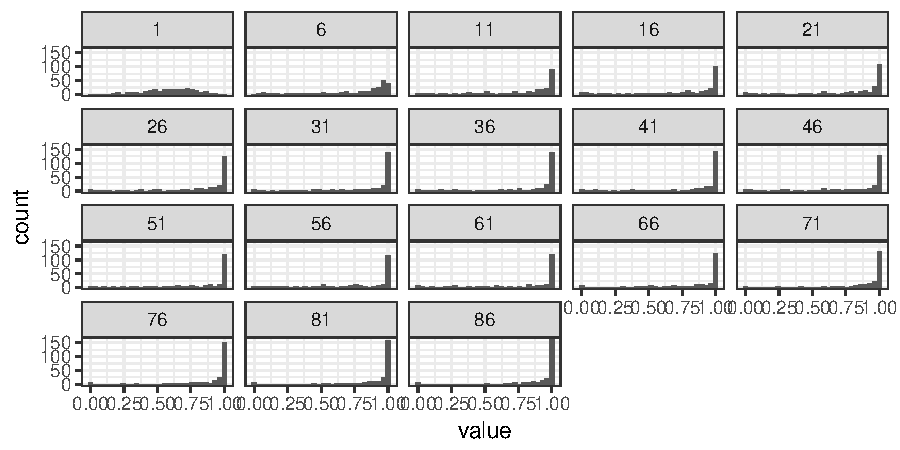
\includegraphics[scale=.55]{wordFormationExample.pdf}}
%{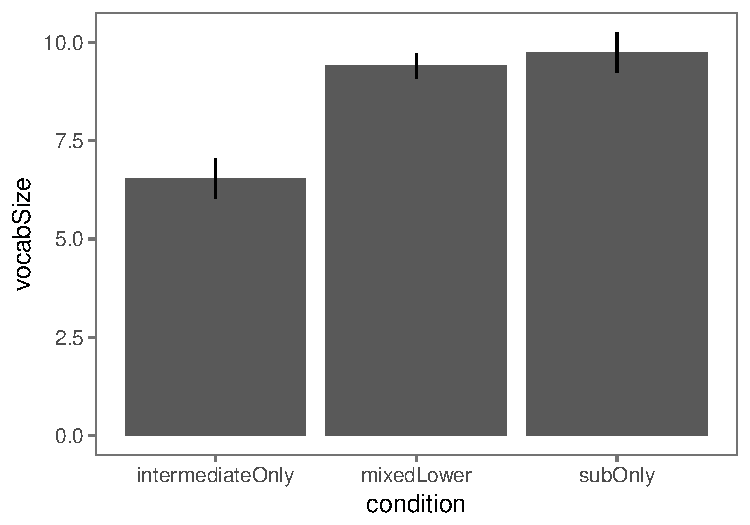
\includegraphics[scale=.64]{lexiconSize.pdf}}
{\caption{{\footnotesize \todo[inline]{TODO: placeholder for more schematic figure showing example of how lexicon inference changes as we see more and more data; would ideally make clear effect of different contexts}  \label{fig:modelSchematic}}}}
\end{center}
\end{figure}


\subsection{Examining early time course}

\todo[inline]{TODO: show predictive accuracy trajectories for each condition; walk through examples of early rounds in different contexts; show timecourse of abstractions, e.g. are initially specific terms extended or are initially abstract terms narrowed? Report posterior predictive accuracy that actually accomodates the data; use >0.5 threshold, maybe with some learned decision offset. Collapse into quartiles instead of diffusion. Distribution over word extensions at each point in time, i.e. change in lexicon. Do you tend to move from big to small or small to big quarter-to-quarter. }

\begin{figure}[t]
\begin{center}
{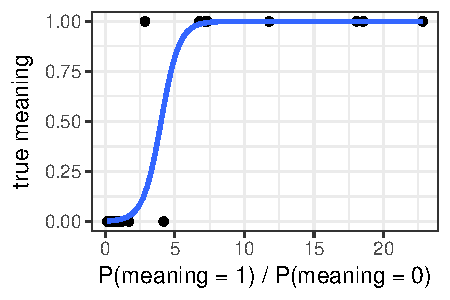
\includegraphics[scale=.94]{postTestPrediction.pdf}}
%{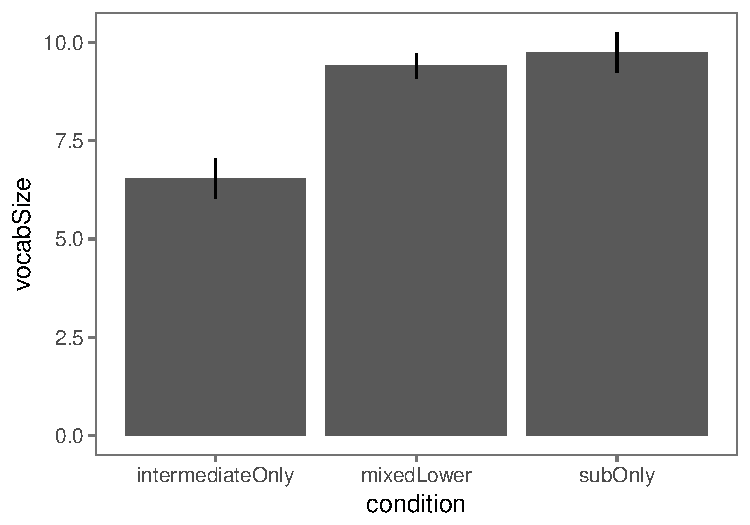
\includegraphics[scale=.64]{lexiconSize.pdf}}
{\caption{{\footnotesize \todo[inline]{TODO: placeholder for plot showing predictions for all games (currently only one game\dots)}  \label{fig:postTestPrediction}}}}
\end{center}
\end{figure}


\section{Discussion}

How do abstractions emerge in the lexicon? Motivated by recent computational accounts of lexical adaptation at both global and local time scales, we hypothesized that while constrained communicative contexts would favor informative one-to-one object-word mappings, under-constrained contexts would allow language users to get away with extending meanings to broader features. By manipulating the statistics of communicative context in a repeated reference game with novel labels, we found both qualitative behavioral evidence and finer-grained model-based evidence for pragmatic influences on convention formation.

These results also help illuminate the relationship between our concepts and words, which are often treated interchangeably. While our individual mental representations of taxonomies are indpendently adaptive to the natural perceptual structure of the world (Rosch et al, 1976; Mervis \& Rosch ,1981; Murphy \& Smith, 1982), it is far from inevitable that all levels of these conceptual hierarchies become conventionalized as lexical items. There are many perfectly natural concepts that are not represented by distinct words in the English language: for instance, we do not have words for each individual tree in our yards, or for abstract but ad-hoc concepts like \emph{things to sell at a garage sale} (Barsalou, 1983). Indeed, English speakers are often fascinated by difficult to express concepts like ``hygge'' or ``tartle'' that are lexicalized as simple words in foreign languages.

While we showed how abstractions emerge even in a task requiring only reference to individual object, there are other clear functional advantages to having abstract terms in the lexicon. For one, they allow speakers to efficiently refer to large, potentially infinite, sets of things, and make generalizations about categories, e.g. ``Dogs bark'' (Tessler \& Goodman, 2016) \dots

\todo[inline]{Should we comment on some methodlogical things people put in the `strategy' box? e.g. some people seem to be taking notes or using sound-symbolic associations like "nogo" to mean "red" (not a problem; should just help memory or help make initial meanings not entirely arbitrary but shouldn't change contextual demands\dots)}

\todo[inline]{Some broader comment connecting to/contrasting with other cognitive theories of what's going on here? e.g. (1) not a simple associative learning account, where people just store memory traces of word-object co-occurances (can't account for context effects). (2) elaborates on Xu \& Tenenbaum (2007) story by introducing contextual pressures. (3) maybe some whole object inductive bias (Markman, 1990) explaining prevalence of specific terms even in intermediate condition (or are  basic-level terms are learned earlier, since most reference to \emph{dog}s is in `intermediate-neighbor` contexts, or higher}

We showed how abstractions become lexicalized when participants were restricted to single-word utterances, but how the lexicalization of nominal terms trades off with compositionality is an open question. Following the same argument, we expect that labels become lexicalized when the cost incurred by frequently using a compositional construction exceeds the cost of adding an additional word to the lexicon. 

Our separate minds may organize the world into meaningful conceptual hierarchies but our shared language only evolves to reflect this structure when it is communicatively relevant. 


\section{\bf Acknowledgments}
\small
This work was supported by ONR grant N00014-13-1-0788 and a James S. McDonnell Foundation Scholar Award to NDG. RXDH was supported by the Stanford Graduate Fellowship and the National Science Foundation Graduate Research Fellowship under Grant No. DGE-114747.

\bibliographystyle{apacite}

\setlength{\bibleftmargin}{.125in}
\setlength{\bibindent}{-\bibleftmargin}

\bibliography{bibs}


\end{document}